\Subsection{Prototipo Nido-Sustrato}
\label{subsection:nido-sustrato}
Para la construcción del prototipo del nido se tuvo en cuenta que el sustrato debe ser madera. Para las medidas se tuvieron en cuenta las dimensiones promedio de un nido de carpintero \cite{ref:PaperValeriaOjeda}.

Por otro lado para alojar y proteger la electrónica se contempló el desarrollo de encapsulados. Primero se trabajó con la \rspi y sus complementos. Se adaptó un diseño existente agrandando su tamaño para que puedan introducirse las placas requeridas, se extendieron y fabricaron ranuras para el conexionado y se agregó un soporte que permita atornillar el conjunto. Para los sensores, se diseñó otro contenedor el cual contempla ranuras para que la cámara y los demás componentes estén en contacto con el exterior y ranuras para el conexionado con la \rpi.

Es así que el diseño del prototipo de nido se puede observar en los planos especificados en las Figuras (\ref{fig:base_nido_plano}), (\ref{fig:tapa_nido_plano}) y (\ref{fig:explotado_nido_plano}), mientras que los encapsulados se encuentran en las Figuras (\ref{fig:RpiCasingBottom}), (\ref{fig:RpiCasingTop}), (\ref{fig:BasePlano}) y (\ref{fig:TapaPlano}).

Finalmente en la Figura (\ref{fig:caja_prototipo}) se puede observar el prototipo del producto montado sobre un nido artificial construido con madera. En dicha imagen se puede observar un elemento extra cerca del encapsulado de la \rspi. Este complemento puede ser observado con mayor detalle en la Figura (\ref{fig:Charger}). La justificación del elemento se explica más adelante.
\begin{figure}[H]
	\centering	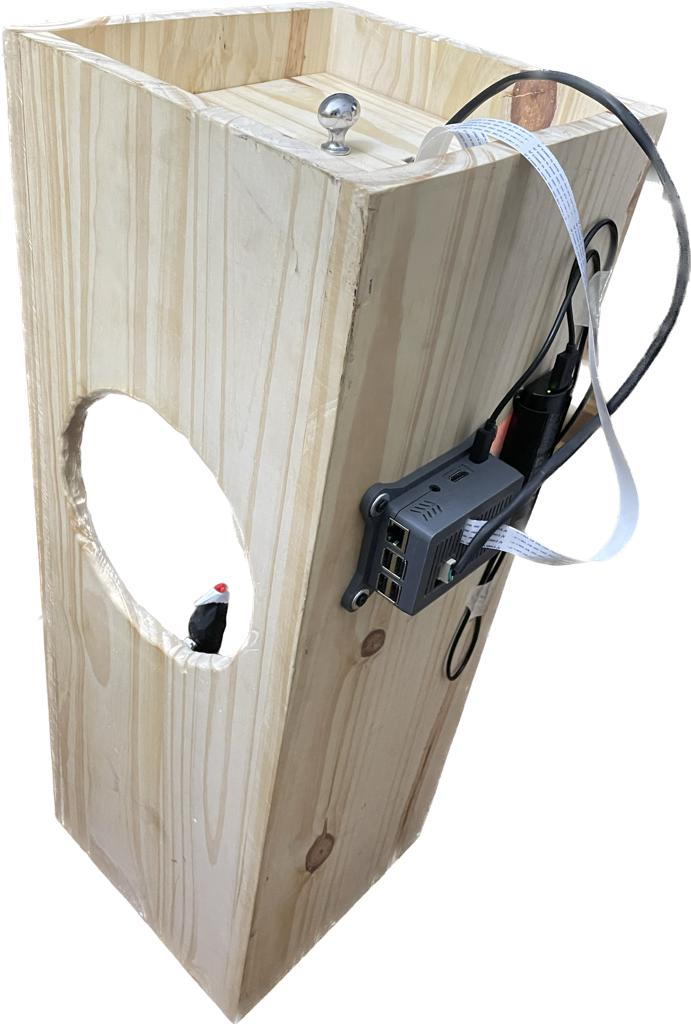
\includegraphics[width=0.4\linewidth,page=1]{ImagenesConstruccion del prototipo/caja_prototipo_2}		
	\caption{Prototipo del producto montado sobre un nido artificial construido con madera.}
	\label{fig:caja_prototipo}
\end{figure}

\Subsection{Prototipo Nido-Electrónica}

\Subsubsection{\rspi}
Para el prototipo se utiliza una \rspi 3B, sobre la cual se desarrollan los \textit{drivers} de comunicación con los diversos sensores. Además se confeccionó un \textit{shield} (encapsulado), el cuál realiza el acondicionamiento de las señales e interfaz para la placa de sensores, como se observa en la Figura (\ref{fig:shield}).
\begin{figure}[H]
	\centering	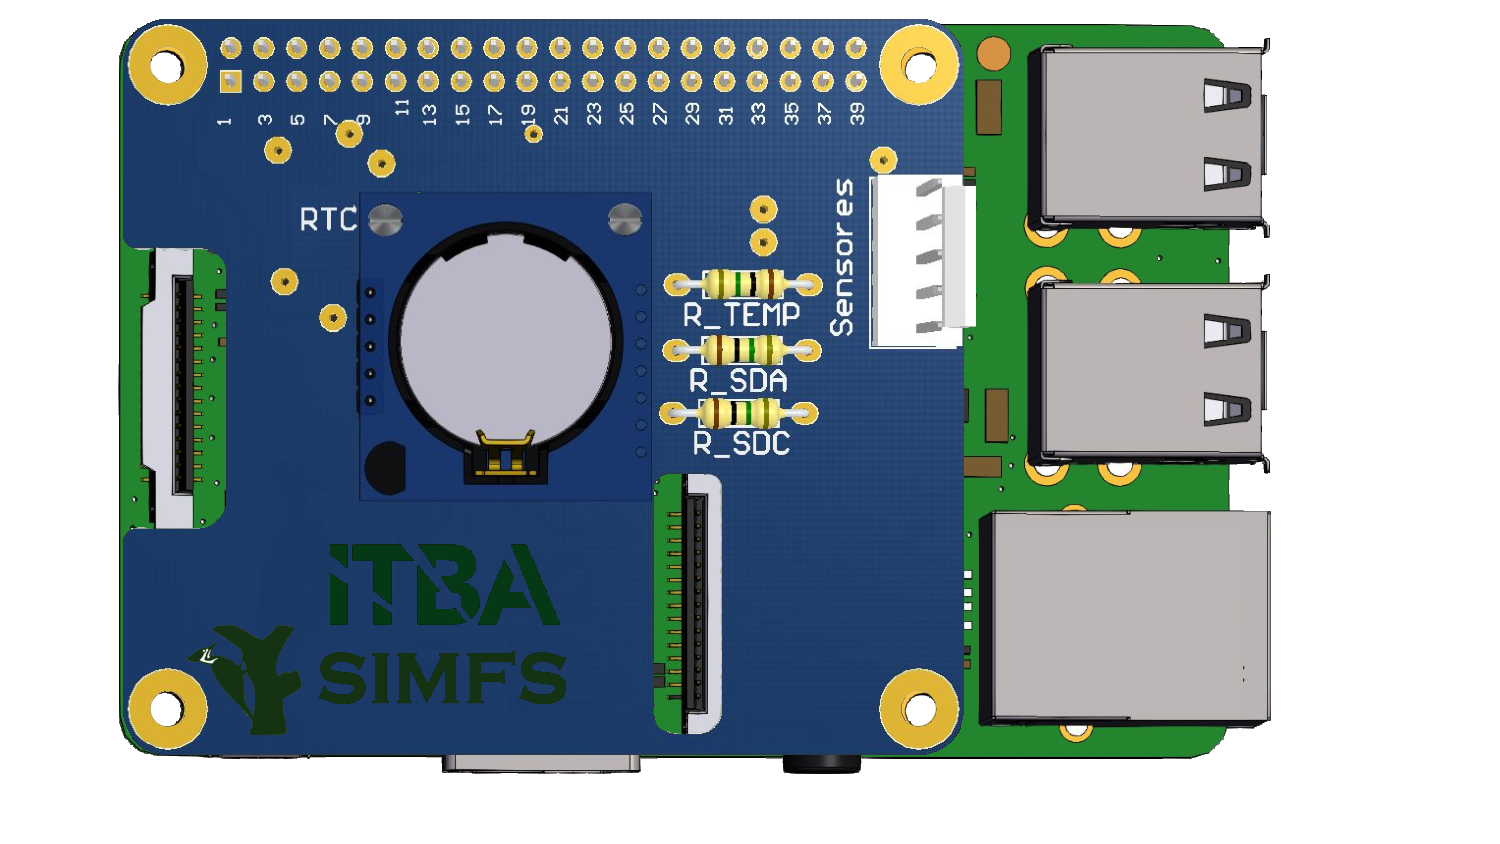
\includegraphics[width=0.6\linewidth,page=1]{ImagenesConstruccion del prototipo/shieldSensor}		
	\caption{\rspi y su \textit{shield}.}
	\label{fig:shield}
\end{figure}

\begin{figure}[H]
\centering
    	\begin{subfigure}{0.4\textwidth}
        	\centering
        	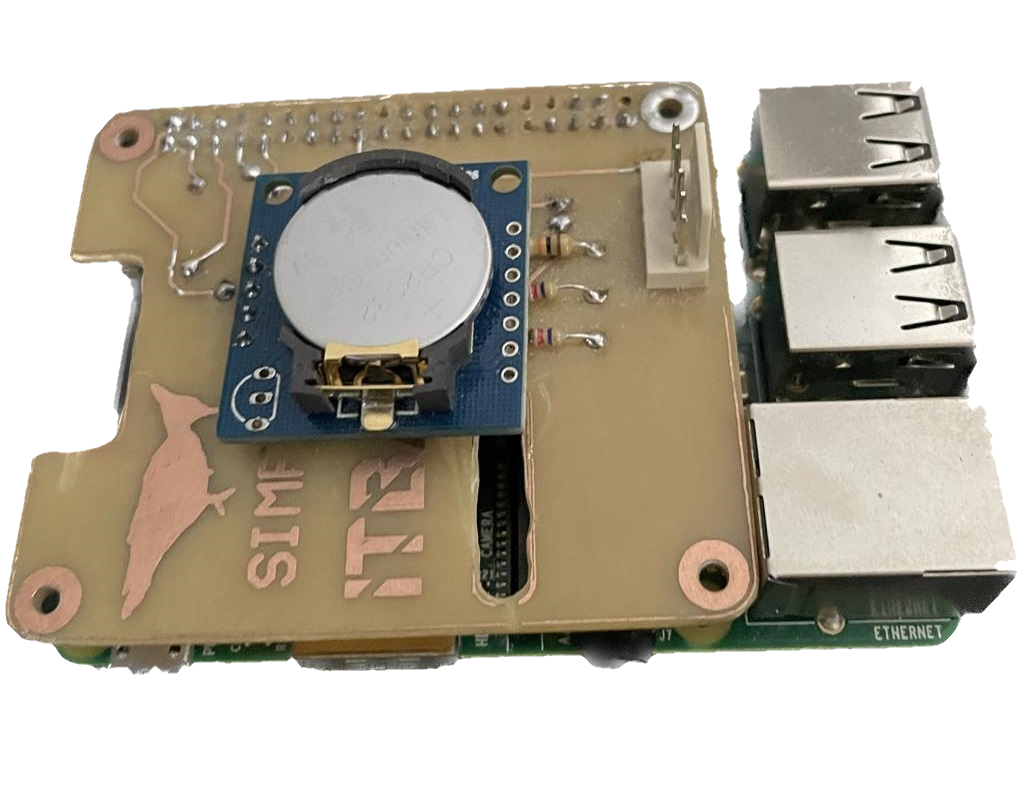
\includegraphics[width=\linewidth]{ImagenesConstruccion del prototipo/rpiyshield_prototipo}		
			\caption{\rspi y su shield implementado.}
			\label{fig:rpiyshield_prototipo}
        \end{subfigure}\hspace*{2cm}
        \begin{subfigure}{0.4\textwidth}
        	\centering
        	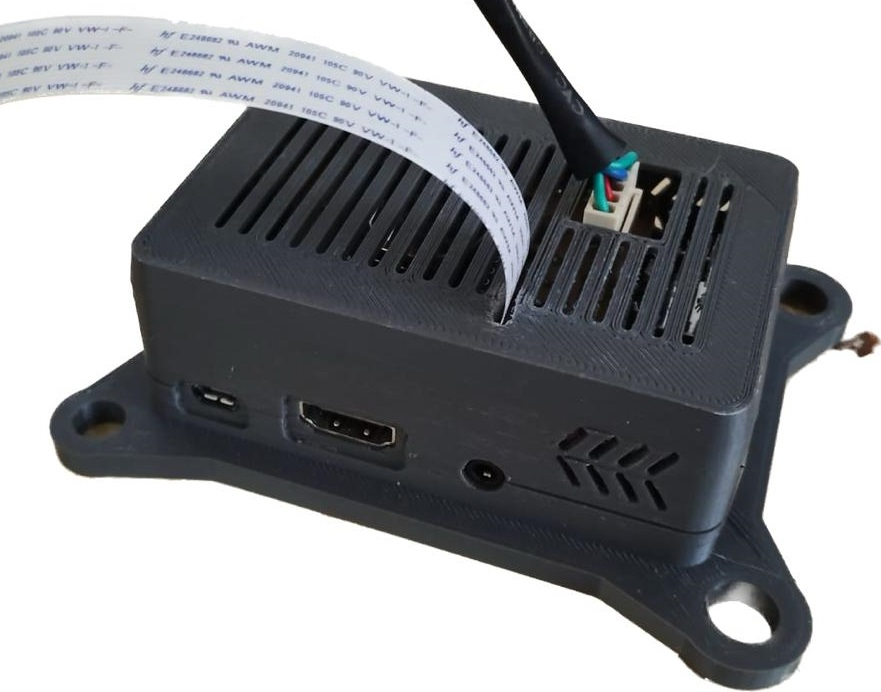
\includegraphics[width=\linewidth]{ImagenesConstruccion del prototipo/rpiyshield_encapsulado_prototipo}
        	\caption{Encapsulado de la \rspi y su \textit{shield} implementado.}
			\label{fig:casing_rpi}
        \end{subfigure}
	\caption{Construcción de la unidad de procesamiento del prototipo.}
	\label{fig:up_prototipo}
\end{figure}

\Subsubsection{Sensores}
En cuanto a los sensores se diseña una placa que se ubica en la bóveda del nido, la cual reúne todos los sensores necesarios, y ofrece una interfaz con la placa \textit{shield}.
\begin{figure}[H]
	\centering
	\includegraphics[width=0.6\linewidth,page=2]{ImagenesConstruccion del prototipo/shieldSensor}		
	\caption{Placa de sensores.}
	\label{fig:sens}
\end{figure}

\begin{figure}[H]
\centering
    	\begin{subfigure}{0.3\textwidth}
        	\centering
        	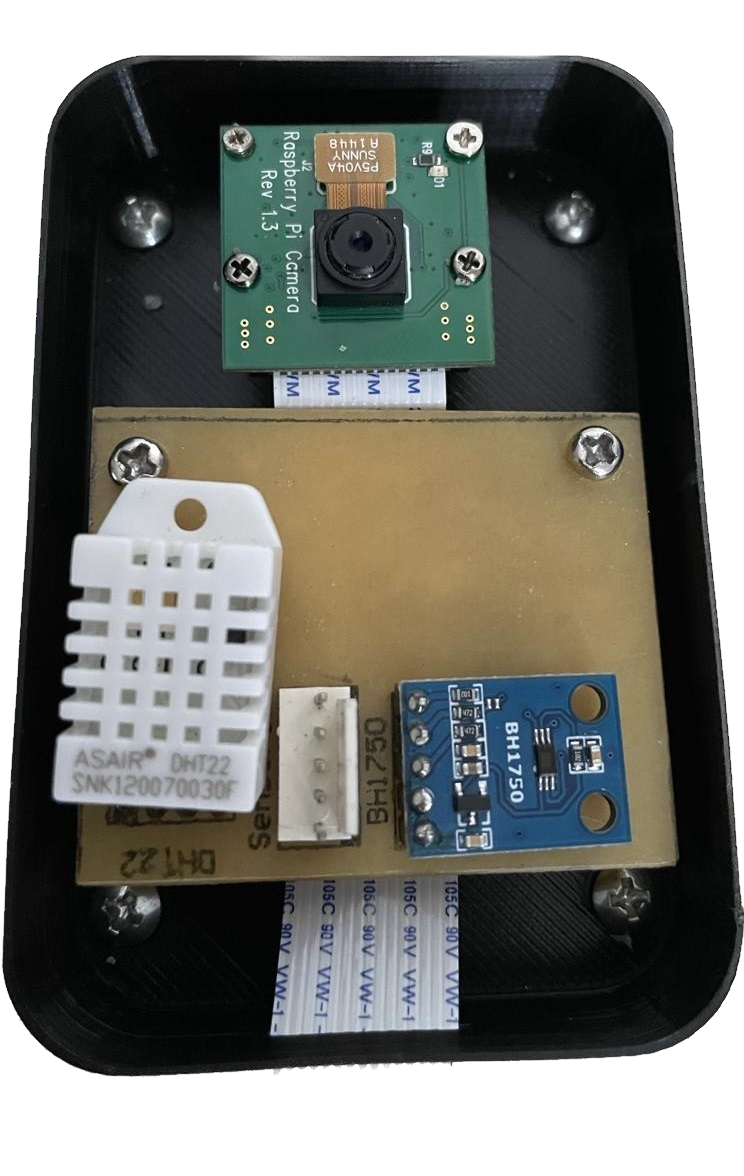
\includegraphics[width=\linewidth]{ImagenesConstruccion del prototipo/sensores_prototipo}		
			\caption{Placa de sensores implementada.}
			\label{fig:sensores_prototipo}
        \end{subfigure}\hspace*{2cm}
        \begin{subfigure}{0.3\textwidth}
        	\centering
        	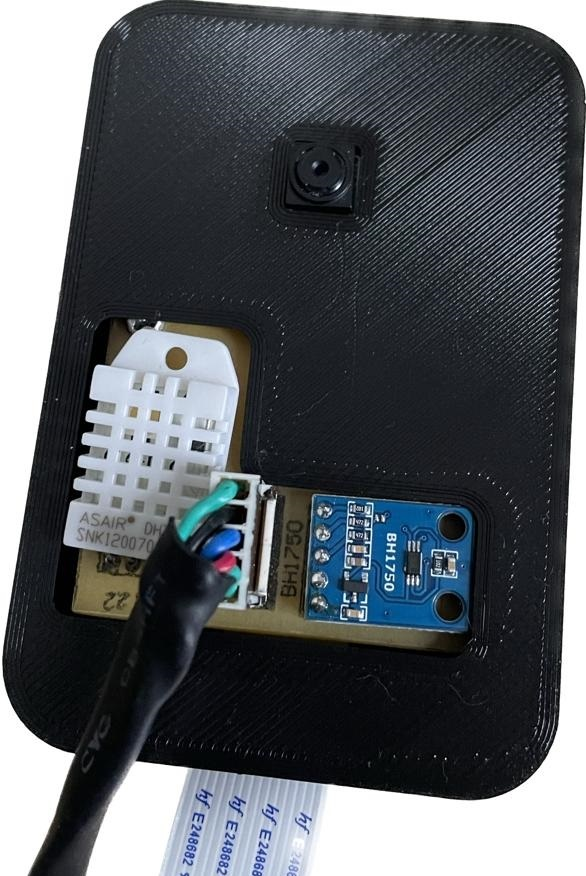
\includegraphics[width=\linewidth]{ImagenesConstruccion del prototipo/sensores_encapsulado_prototipo_alt}
        	\caption{Encapsulado de la placa de sensores implementada.}
			\label{fig:sensores_encapsulado_prototipo_alt}
        \end{subfigure}
	\caption{Construcción de la placa de sensores y su encapsulado para el prototipo.}
	\label{fig:sensores_prototipado}
\end{figure}

\Subsection{Prototipo Nido-Potencia}
\label{subsection:nido-potencia}
Para el prototipo del sistema de potencia del nido, se cuenta con la batería \href{https://enertik.ar/taiyo-tyd12-33-bateria-electrolito-absorbido-ciclo-profundo-12v-33ah}{TAIYO TYD12-33} de plomo-ácido de ciclo profundo AGM de $33 \ Ah$ y la fuente de tensión \href{https://www.itech.sh/en/product/dc-power-supply/IT6500.html}{ITECH IT6536C} con capacidad de simular la curva de tensión-corriente de un panel solar.
\begin{figure}[H]
	\centering
    	\begin{subfigure}{0.3\textwidth}
        	\centering
        	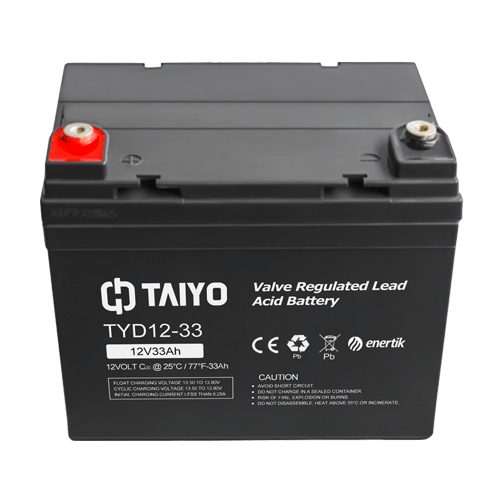
\includegraphics[width=\linewidth]{ImagenesConstruccion del prototipo/bateria_prototipo}		
			\caption{Batería utilizada en la construcción del prototipo.}
			\label{fig:bateria_prototipo}
        \end{subfigure}\hspace*{2cm}
        \begin{subfigure}{0.3\textwidth}
        	\centering
        	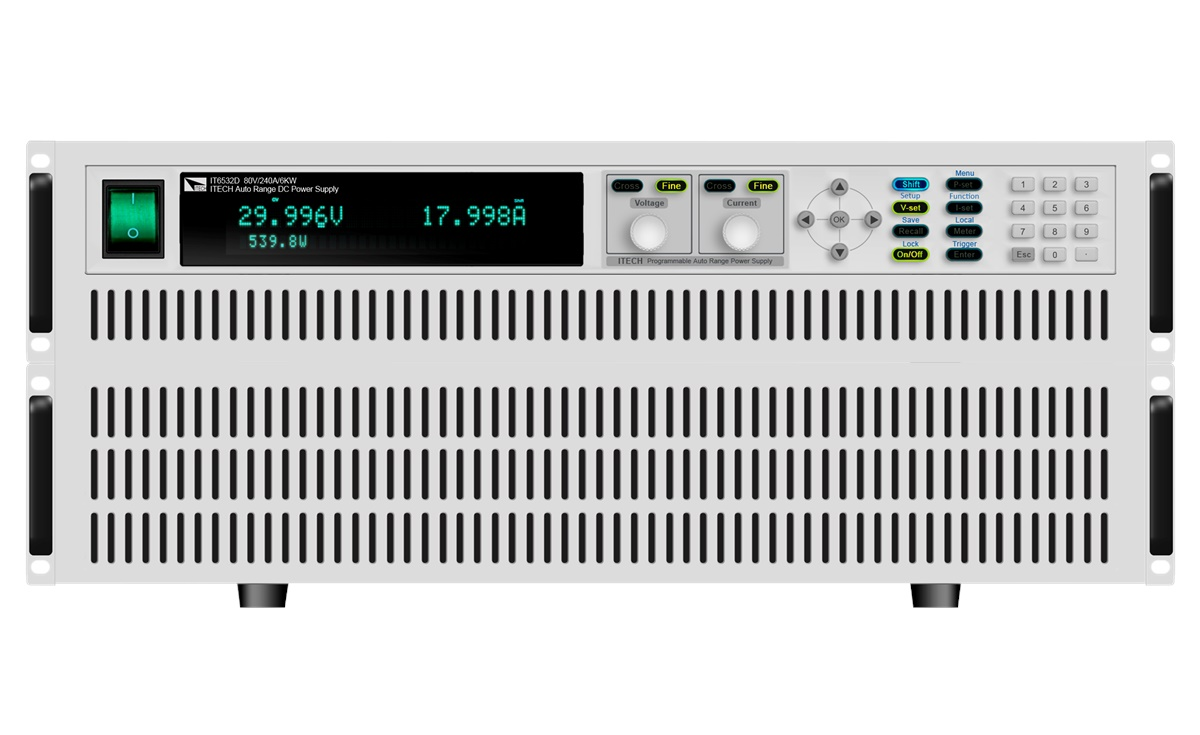
\includegraphics[width=\linewidth]{ImagenesConstruccion del prototipo/fuente_prototipo}
        	\caption{Fuente de tensión con capacidad de simular la curva tensión-corriente de un panel solar utilizado en el prototipo.}
			\label{fig:fuente_prototipo}
        \end{subfigure}
	\caption{Comparación entre el uso del filtro de luminosidad.}
	\label{fig:elementos_prototipo}
\end{figure}

Se utiliza el \textit{Solar Power Manager} \href{https://wiki.dfrobot.com/Solar_Power_Manager_For_12V_Lead-Acid_Battery_SKU__DFR0580}{DFR0580} que se encarga de extraer eficientemente la energía generada por el panel solar mediante el algoritmo de MPPT, cargar la batería y proveer las salidas de alimentación acondicionadas para la \rpi.

Alternativamente, para disminuir el tamaño del prototipo, se reemplaza la fuente de alimentación del sistema. Este cambio se realiza únicamente en aquellos procesos en los cuales no influya utilizar otro sistema como batería, como son los bancos de prueba o el uso del prototipo en ambientes de desarrollo que no abarcan el sistema de abastecimiento, entre otros.

Se opta por utilizar un \textit{Power Bank} (batería externa) que cumpla con los requisitos de tensión y corriente necesarios. El dispositivo elegido para esta tarea es el cargador \href{https://www.sony.com/electronics/support/res/manuals/W000/W0002536M.pdf}{CP-V3} de la empresa \textit{Sony}.

Las razones por las cuales se decidió utilizar dicha tecnología como alternativa es porque posee alta portabilidad, un tamaño reducido, es independiente de la red eléctrica, brinda una señal de alimentación estable y es fácilmente recargable. 

Como se mencionó en la Sección (\ref{subsection:nido-sustrato}), este elemento se adosa al nido artificial mediante el soporte presentado en la Figura (\ref{fig:Charger}). 

\Subsection{Prototipo Nido-Comunicaciones }
Existen dos tipos de comunicación que se realiza en el prototipo: la encargada de \nodered para la comunicación con usuarios y la comunicación con la base principal de seguimiento para la recolección de datos del ave.
